\section{Macros}

\section{Notation}
\begin{itemize}
	\item By \emph{goal} or \emph{problem} or \emph{task} we mean the overall task of the thesis, which is develop a machine learning model suitable for predicting prices on the financial market, based on a history of data.
\end{itemize}

\section{Datasets}
Here we describe the various time series datasets we used for the training and testing of our models. In the below table, the columns describe the following:
\begin{itemize}
	\item \textbf{Name:} the name of the dataset.
	\item \textbf{Source:} the source from where we took the dataset - most we received from AI Investments company. For others we include a link or a way to access and download the dataset.
	      % \item \textbf{Collection method:} a description of how the data in the dataset was gathered and over what time span.
	      % \item \textbf{Motivation:} a description of what the data in the dataset represent, what their purpose is, how they were gathered and why it is valuable to our research.
	\item \textbf{Number of datapoints:} a description of how many datapoints the dataset contains, how many features each datapoints has and the overall size of the file.
	\item \textbf{Datapoints used:} how many of these datapoints were used in model training (these are taken from the end of the dataset).
	\item \textbf{Time step:} what is the time difference in the Date column between subsequent datapoints.
	      % \item \textbf{Features:} a description of the features each datapoint of the dataset has and what the features represent.
	      % \item \textbf{Additional characteristics:} a description of the features and drawbacks of the overall dataset e.g. how dependent are the features between themselves.
	      % \item \textbf{Plot:} a plot of the numeric features of the dataset, its visual representation.
\end{itemize}



\begin{center}
	\begin{tabular}{||p{0.15\linewidth} ||p{0.2\linewidth} | c | p{0.15\linewidth} | c | c ||}
		\hline
		\multicolumn{6}{|c|}{Datasets summary}                                                                                                         \\
		\hline
		Dataset name & Short description                      & Source                           & Number of datapoints & Datapoints used & Time step  \\ [0.5ex]
		\hline\hline
		AAPL         & Apple stock prices                     & Online \cite{apple_source}       & 10943                & 10000           & 1 day      \\
		\hline
		BTCUSD       & Rates of Bitcoin in US Dollars         & AI Investments                   & 40450                & 40450           & 1 hour     \\
		\hline
		EURUSD       & Rates of Euro in US Dollars            & AI Investments                   & 117397               & 117397          & 1 hour     \\
		\hline
		GBPCAD       & Rates  of GB Pound in Canadian Dollars & AI Investments                   & 117423               & 117423          & 1 hour     \\
		\hline
		GBPTRY       & Rates of GB Pound in Turkish Lires     & AI Investments                   & 35965                & 35965           & 1 hour     \\
		\hline
		US500        & US500 stock index                      & AI Investments                   & 118023               & 118023          & 1 hour     \\
		\hline
		Electricity  & Electricity consumption                & Online \cite{electricity_source} & 26304                & 26304           & 15 minutes \\[1ex]
		\hline
	\end{tabular}
\end{center}

\subsection{Explanation of the datasets}
All except for the Electricity dataset are market time series - they have the following features:
\begin{itemize}
	\item \textbf{date} - The time at which the datapoint was recorded.
	\item \textbf{close} - Closing price within given time interval.
	\item \textbf{high} - Highest price within given time interval.
	\item \textbf{low} - Lowest Price within given time interval.
	\item \textbf{open} - Opening price within given time interval.
	\item \textbf{volume} - Volume of stock traded.
	\item \textbf{adjClose} - Closing price within given time interval, modified to account for dividends, stock splits, etc., to better reflect stock value.
\end{itemize}
Our target column was the \textbf{close} column. All others were discarded.


The Electricity dataset in addition to the \textbf{date} column has 370 columns, which correspond to different energy consumption clients. Every datapoint records the energy consumption for the timestep period at each of these clients. For the target column, we chose the 127th column.
This dataset serves to check whether the approach to market time-series generalises to other types of time-series.

In all experiments, the dataset used was divided into 3 parts: the first 70\% was used in the testing of the model, then 10\% was used in its validation, and 20\% was used for testing.


\section{Metrics}

\subsection{Mean Squared Error}
The \emph{Mean Squared Error} (MSE) is a metric used during training of machine learning model, especially in regression tasks. It quantifies how close a model's predictions are to the actual values.

\subsubsection{Definition}
MSE calculates the average of the squares of the errors. The error is the difference between the values (\(\hat{y}_i\)) predicted by the model and the actual values (\(y_i\)).

\subsubsection{Calculation Steps}
The metric is computed as follows:
\begin{enumerate}
	\item for each prediction the error is computed by subtracting the predicted value from the actual value;
	\item each error is then squared in order to ensure that positive and negative errors do not cancel each other out and in order to emphasize larger errors;
	\item the average of these squared errors is then computed to obtain the MSE.
\end{enumerate}

\subsubsection{Mathematical Formulation}
The mathematical formula for MSE is given by
\begin{equation}
	MSE = \frac{1}{n} \sum_{i=1}^{n} (y_i - \hat{y}_i)^2,
\end{equation}
where:
\begin{itemize}
	\item \(n\) is the number of data points;
	\item \(y_i\) is the actual value for the \(i\)th datapoint;
	\item \(\hat{y}_i\) is the predicted value for the \(i\)th datapoint.
\end{itemize}

\subsubsection{Interpretation}
\begin{itemize}
	\item MSE is a non-negative number where a value of 0 indicates perfect predictions.
	\item Larger MSE values indicate worse model performance.
	\item MSE emphasizes larger errors due to the squaring of each term, which can be both advantageous and disadvantageous depending on the application.
\end{itemize}


\subsection{Accuracy metric}
The \emph{Accuracy} metric measures correctness of class predictions of a model. In the context of time series prediction, it is measured as follows.

When we predict the value \(a_{i+k}\) based on values \([a_{i-n}, a_i]\) in a time series, we
\begin{enumerate}
	\item classify the prediction \(\hat{a}_{i+k}\) into a binary up/down class, based on whether the predicted value is higher or lower then the last known one:
	      \[
		      \mathsf{class}(\hat{a}_{i+k}) =
		      \begin{cases}
			      1, & \text{if } \hat{a}_{i+k} \ge a_i \\
			      0, & \text{otherwise}
		      \end{cases}
	      \]
	\item We then classify the value actually observed \(a_{i+k}\) in the same way.
	\item Subsequently we calculate the fraction of the times when such predictions were correct, i.e. \(\mathsf{class}(\hat{a}_{i+k}) = \mathsf{class}(a_{i+k})\).
	\item This yields an \emph{accuracy} score, between 0 and 1: \(0 \leq \frac{\sum_{i=1}^N[\mathsf{class}(\hat{a}_{i+k}) = \mathsf{class}(a_{i+k})]}{N} \leq 1\). \footnote{Here for \(N\) predictions.}
\end{enumerate}

% TODO: more elaborate description

% TODO: describe how we measure accuracy























% \subsection{House sales}
% \begin{itemize}
% 	\item \textbf{Source:} House Property Sales Time Series (raw\_sales.csv) :\\ https://www.kaggle.com/datasets/htagholdings/property-sales
% 	\item \textbf{Collection method:} Property sales data was gathered for the 2007-2019 period for one specific region \footnote{The region in question was not specified in the description of the dataset.}
% 	\item \textbf{Motivation:} A simple dataset for the basic models. A proper, manageable size, once filtered by property and number of bedrooms. Has very few features, making it easier to understand and process.
% 	\item \textbf{Size:} Consists of 29600 datapoints. Once filtered for property being house, number of bedrooms equal to 3, around 11300 datapoints remain.
% 	\item \textbf{Features:} The dataset has very few features. Every datapoint consists of:
% 	      \begin{itemize}
% 		      \item \textbf{datesold}: Date at which the sale was made.
% 		      \item \textbf{postcode}: 4 digit postcode of the suburb where the property was sold (given for reference only).
% 		      \item \textbf{price}: Price for which the property was sold.
% 		      \item \textbf{propertyType}: Property type i.e. house or unit.
% 		      \item \textbf{bedrooms}: Number of bedrooms: 1, 2, 3, 4 or 5.
% 	      \end{itemize}
% 	      The dataset was filtered by propertyType and bedrooms, and the postcode was discarded.

% 	      % może inaczej nazwać, dyskusja
% 	\item \textbf{Characteristic:} The prices rise with time, therefore models might easily learn to always predict "up".

% 	\item \textbf{Plot:} Below is the plot of prices with respect to time for properties with different numbers of bedrooms.
% 	      \begin{figure}[h!]
% 		      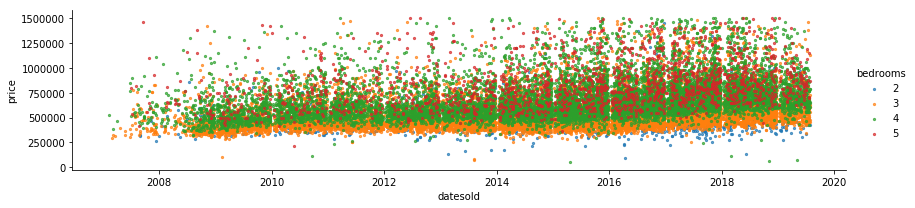
\includegraphics[width=\linewidth]{"pictures/house_sales_graph.png"}
% 		      \caption{A plot of the House Sales dataset.}
% 		      \label{fig:house_sales_graph}
% 	      \end{figure}
% \end{itemize}
% \subsection{Apple}
% \begin{itemize}
% 	\item \textbf{Source:} Apple Stock Prices \\ https://finance.yahoo.com/quote/AAPL/history/
% 	\item \textbf{Collection method:} Collected from the stock market (probably).
% 	\item \textbf{Motivation:} Even more features then the Google Stock dataset, more interesting.
% 	\item \textbf{Size:} The dataset consists of 1258 datapoints.
% 	\item \textbf{Features:} Every datapoint has the following features
% 	      \begin{itemize}
% 		      \item \textbf{close} - Closing price
% 		      \item \textbf{high} - Highest price of the day
% 		      \item \textbf{low} - Lowest Price of the day
% 		      \item \textbf{open} - Opening price of the day
% 		      \item \textbf{volume} - Volume of stock traded
% 		      \item \textbf{adjClose} - Closing price of the day, modified to account for dividends, stock splits, etc., to better reflect stock value.
% 		      \item \textbf{adjHigh} - Highest price of the day, modified to account for dividends, stock splits, etc., to better reflect stock value.
% 		      \item \textbf{adjOpen} - Opening price of the day, modified to account for dividends, stock splits, etc., to better reflect stock value.
% 		      \item \textbf{adjVolume} - Trading volume of the day, modified to account for dividends, stock splits, etc., to better reflect stock value.
% 		      \item \textbf{divCash} - Cash dividend - the amount of money payed per share to the stockholder.
% 		      \item \textbf{splitFactor} - Stock split factor - the ratio used to adjust number of shares and their prices during a stock split.
% 	      \end{itemize}
% 	      % \item \textbf{Characteristic:}
% 	      % \item \textbf{Plot:}
% \end{itemize}
% \subsection{BTCUSD}
% \begin{itemize}
% 	\item \textbf{Source:}
% 	\item \textbf{Motivation:}
% 	\item \textbf{Size:}
% 	\item \textbf{Features:}
% 	\item \textbf{Collection method:}
% 	\item \textbf{Quality:}
% 	\item \textbf{Plot:}
% \end{itemize}
% \subsection{EURUSD}
% \begin{itemize}
% 	\item \textbf{Source:}
% 	\item \textbf{Motivation:}
% 	\item \textbf{Size:}
% 	\item \textbf{Features:}
% 	\item \textbf{Collection method:}
% 	\item \textbf{Quality:}
% 	\item \textbf{Plot:}
% \end{itemize}
% \subsection{GBPCAD}
% \begin{itemize}
% 	\item \textbf{Source:}
% 	\item \textbf{Motivation:}
% 	\item \textbf{Size:}
% 	\item \textbf{Features:}
% 	\item \textbf{Collection method:}
% 	\item \textbf{Quality:}
% 	\item \textbf{Plot:}
% \end{itemize}
% \subsection{GBPTRY}
% \begin{itemize}
% 	\item \textbf{Source:}
% 	\item \textbf{Motivation:}
% 	\item \textbf{Size:}
% 	\item \textbf{Features:}
% 	\item \textbf{Collection method:}
% 	\item \textbf{Quality:}
% 	\item \textbf{Plot:}
% \end{itemize}
% \subsection{Electricity}
% \begin{itemize}
% 	\item \textbf{Source:}
% 	\item \textbf{Motivation:}
% 	\item \textbf{Size:}
% 	\item \textbf{Features:}
% 	\item \textbf{Collection method:}
% 	\item \textbf{Quality:}
% 	\item \textbf{Plot:}
% \end{itemize}
% \subsection{US500}
% \begin{itemize}
% 	\item \textbf{Source:}
% 	\item \textbf{Motivation:}
% 	\item \textbf{Size:}
% 	\item \textbf{Features:}
% 	\item \textbf{Collection method:}
% 	\item \textbf{Quality:}
% 	\item \textbf{Plot:}
% \end{itemize}
% \subsection{Google Stock}
% \begin{itemize}
% 	\item \textbf{Source:} Google Stock Dataset \\ https://www.kaggle.com/datasets/r1shabhgupta/google-stock-price-daily-weekly-and-monthly-2023/data
% 	\item \textbf{Collection method:} We suspect this data was collected from the stock market (the source does not specify this). Has daily data and weekly and monthly summaries.
% 	\item \textbf{Motivation:} More complex dataset, multiple time series numeric features, but fewer datapoints.
% 	\item \textbf{Size:} Daily set has 2510 datapoints. Weekly set has 520 datapoints. Monthly set has 120 datapoints.
% 	\item \textbf{Features:} Every datapoint has the following features:
% 	      \begin{itemize}
% 		      \item \textbf{Date}: the date on which the stock price was recorded.
% 		      \item \textbf{Price}: the opening price of the stock on the given date.
% 		      \item \textbf{High}: the highest price at which the stock was traded during the day.
% 		      \item \textbf{Low}: the lowest price at which the stock was traded during the day.
% 		      \item \textbf{Close}: the closing price of the stock on the given date.
% 		      \item \textbf{Volume}: the total number of shares traded on the given date.
% 		      \item \textbf{Adj Close}: the close price modified to account for dividends, stock splits, etc., to better reflect stock value.
% 	      \end{itemize}
% 	\item \textbf{Characteristic:}
% 	\item \textbf{Plot:}
% \end{itemize}
% \subsection{Gold}
% \begin{itemize}
% 	\item \textbf{Source:} Gold rates \\ https://www.kaggle.com/datasets/hemil26/gold-rates-1985-jan-2022
% 	\item \textbf{Collection method:} This data was collected from https://www.gold.org/goldhub and then cleaned. Has daily data and annual summaries.
% 	\item \textbf{Motivation:} The dataset contains lots of datapoints and lots of features.
% 	\item \textbf{Size:} Annual dataset has 43 datapoints. Daily dataset has a bit over 10 thousand datapoints.
% 	\item \textbf{Features:} Each datapoint has the following features: date and rates in six curriencies: USD (American), INR (Indian), AED (Arabian), EUR (European), GBP (South Georgian) and CNY (Chinese).
% 	      % \item \textbf{Characteristic:}
% 	      % \item \textbf{Plot:}
% \end{itemize}
% \subsection{Time Series Practice Dataset}
% \begin{itemize}


% 	\item \textbf{Source:} https://www.kaggle.com/datasets/samuelcortinhas/time-series-practice-dataset/data?select=train.csv
% 	\item \textbf{Motivation:} As the Sine dataset it is a fictional dataset to more easily tune LLM training, but more complicated than Sine and significantly larger.
% 	\item \textbf{Size:} This dataset contains 230 thousand simulated time series datapoints covering 10 years (2010-2019).  The are no null values.
% 	\item \textbf{Features:} The features include date, store id, product id and number sold. The train.csv covers the years 2010-2018 and the test.csv covers 2019 only. The are 7 unique stores and 10 unique products.
% 	\item \textbf{Collection method:} This time series data was created using multiple features including various long term trends, year-long seasonality patterns, weekday/weekend effects and noise. Moreover, the products and the stores are supposed to be weakly correlated.

% 	      % \item \textbf{Characteristic:}
% 	      % \item \textbf{Plot:} A simple sine wave.
% \end{itemize}

% \section{What metrics we used}
% Every metric should be described by
% \begin{itemize}
% 	\item \textbf{Definition:} How the metric is defined, what it measures.
% 	\item \textbf{Calculation:} Description of how the metric is calculated.
% 	\item \textbf{Interpretation:} A consideration of what the result of the metric may be interpreted to mean about the model it measures.
% \end{itemize}
% \subsection{Mean Squared Error}

% The Mean Squared Error (MSE) is a metric used for evaluating the accuracy of a machine learning model, especially in regression tasks. It quantifies how close a model's predictions are to the actual values.

% \subsubsection{Definition}
% MSE calculates the average of the squares of the errors. The error is the difference between the values (\(\hat{y}_i\)) predicted by the model and the values (\(y_i\)) it should have predicted.

% \subsubsection{Calculation Steps}
% The metric is computed as follows.
% \begin{enumerate}
% 	\item For each prediction the error is computed by subtracting the predicted value from the actual value.
% 	\item Each error is then squared in order to ensure that positive and negative errors do not cancel each other out and in order to emphasize larger errors.
% 	\item The average of these squared errors is then computed to obtain the MSE.
% \end{enumerate}

% \subsubsection{Mathematical Formulation}
% The mathematical formula for MSE is given by:
% \begin{equation}
% 	MSE = \frac{1}{n} \sum_{i=1}^{n} (y_i - \hat{y}_i)^2
% \end{equation}
% where:
% \begin{itemize}
% 	\item \(n\) is the number of data points,
% 	\item \(y_i\) is the actual value for the \(i\)th datapoint,
% 	\item \(\hat{y}_i\) is the predicted value for the \(i\)th datapoint,
% \end{itemize}

% \subsubsection{Interpretation}
% \begin{itemize}
% 	\item MSE is a non-negative number where a value of 0 indicates perfect predictions.
% 	\item Larger MSE values indicate worse model performance.
% 	\item MSE emphasizes larger errors due to the squaring of each term, which can be both advantageous and disadvantageous depending on the application.
% \end{itemize}

% \subsection{R\(^2\) Score}

% The \(R^2\) score, or the coefficient of determination, is a statistical measure used in regression analysis to assess how well fitted a model is. It indicates the proportion of the variance in the dependent variable that is predictable from the independent variable(s).

% \subsubsection{Definition}
% The \(R^2\) score is defined as the ratio of the variance explained by the model to the total variance. It is a measure of how well the observed outcomes are replicated by the model, based on the proportion of total variation of outcomes explained by the model.

% \subsubsection{Calculation}
% The \(R^2\) score is calculated using the following formula:
% \begin{equation}
% 	R^2 = 1 - \frac{\sum_{i=1}^{n} (y_i - \hat{y}_i)^2}{\sum_{i=1}^{n} (y_i - \overline{y})^2}
% \end{equation}
% where:
% \begin{itemize}
% 	\item \(y_i\) is the actual value for the \(i\)th data point,
% 	\item \(\hat{y}_i\) is the predicted value for the \(i\)th data point,
% 	\item \(\overline{y}\) is the mean of the actual values,
% 	\item \(n\) is the number of data points.
% \end{itemize}

% \subsubsection{Interpretation}
% \begin{itemize}
% 	\item An \(R^2\) score of 1 indicates that the regression model perfectly fits the data.
% 	\item An \(R^2\) score of 0 means that the model does no better, than would a prediction using the mean.
% 	\item Negative \(R^2\) values can occur when the chosen model fits worse than a horizontal line representing the mean of the response.
% \end{itemize}

% \subsubsection{Limitations}
% The \(R^2\) metric has some limitations. It does not necessarily imply causation, nor does a high \(R^2\) score mean that the model is the best choice for prediction. It's also important to note that using more features of the data by the model can artificially inflate the \(R^2\) value, even if those features are not statistically significant.


% \section{How we describe models}
% Below, in the chapter "Other models" we describe several models we tried to use for the task of predicting prices. The descriptions include the following:
% \begin{itemize}
% 	% \item \textbf{Relevant literature:} 
% 	\item \textbf{Description:} a short description of how the model works and how it is trained.
% 	\item \textbf{Motivation:} what the model is usually used for and why we chose to try it out.
% 	\item \textbf{Features and limitations:} some advantages and benefits of the model, as well as its disadvantages and drawbacks.
% 	\item \textbf{Parameters:} the description of the parameters of the model and how they affect its training.
% 	\item \textbf{Metrics:} how we measured the results of the training and testing of the model.
% 	\item \textbf{Data used:} what combinations of parameters of the model we tested and on what datasets we trained and tested the model and how these datasets were divided into training and testing subdatasets.
% 	\item \textbf{Preprocessing:} how the datasets used were preprocessed for training and testing of the model.
% 	\item \textbf{Analysis:} an analysis of our results of our training and testing of the model compared with the results obtained in literature.
% 	\item \textbf{Picture:} a picture or a plot demonstrating the results obtained from testing the model.
% \end{itemize}

% \section{Literature review}
% Literature review contains:
% \begin{itemize}
% 	\item A list of approaches to the problem.
% 	\item For each approach, its basic description and its significance to our goal.
% 	\item Its features and drawbacks compared to our goal.
% 	\item Its differences, when compared to our goal.
% 	\item Whether our own results validated the results of the article.
% \end{itemize}

% notatki:
% opis modelu
% nasze wyniki vs. literatura
% dyskusja - krótka analiza, porównanie z literaturą

% Dla LLM:
% 5 najciekawszych pomysłów, które zadziałały
% 5 najciekawszych pomysłów, które nie zadziałały

% Kryteria oceniania:
% czy nazwa odpowiada treści
% czy ma wstęp, przegląd literatury, własną myśl itp.
% czy jest jasno napisana
% własne wnioski (dlaczego wydaje nam się, że to zadziałało, a to nie)

% wyniki, które trochę przetrwają, coś ciekawego, coś, co ma uniwersalny charakter

% co robić:
% metryki, datasety
% literature review - co tam ma być
